\documentclass{beamer}
\usetheme{CambridgeUS}
\usecolortheme{dolphin}
%themes to test
%Theme to: AnnArbor Antibes Bergen Berkeley Berlin Boadilla boxes CambridgeUS Copenhagen Darmstadt default Dresden Frankfurt Goettingen Hannover Ilmenau JuanLesPins Luebeck Madrid Malmoe Marburg Montpellier PaloAlto Pittsburgh Rochester Singapore Szeged Warsaw
%Color to: albatross beaver beetle crane default dolphin dove fly lily orchid rose seagull seahorse sidebartab structure whale wolverine
%Font to: default professionalfonts serif structurebold structureitalicserif structuresmallcapsserif

%allows picture file insertion into document
\usepackage{graphicx}



\title{Neurologic Manifestations of Hansen's Disease}
\author{Eric W. Robbins}
\date{}
\begin{document}
	\begin{frame}
		\maketitle
	\end{frame}
	\begin{frame}
		\tableofcontents
	\end{frame}
\section{Why Care?}
\subsection{Incidence and Demographics}
	\begin{frame}
		\frametitle{Incidence\textemdash USA}
			\begin{itemize}
				\item New US cases in 2015: 178
				\item 57\% of cases born outside US
				\item Commonest states: TX, LA, AR, MS, FL
				\item Estimated total of 9,140 cases in US
			\end{itemize}
	\end{frame}

	\begin{frame}
		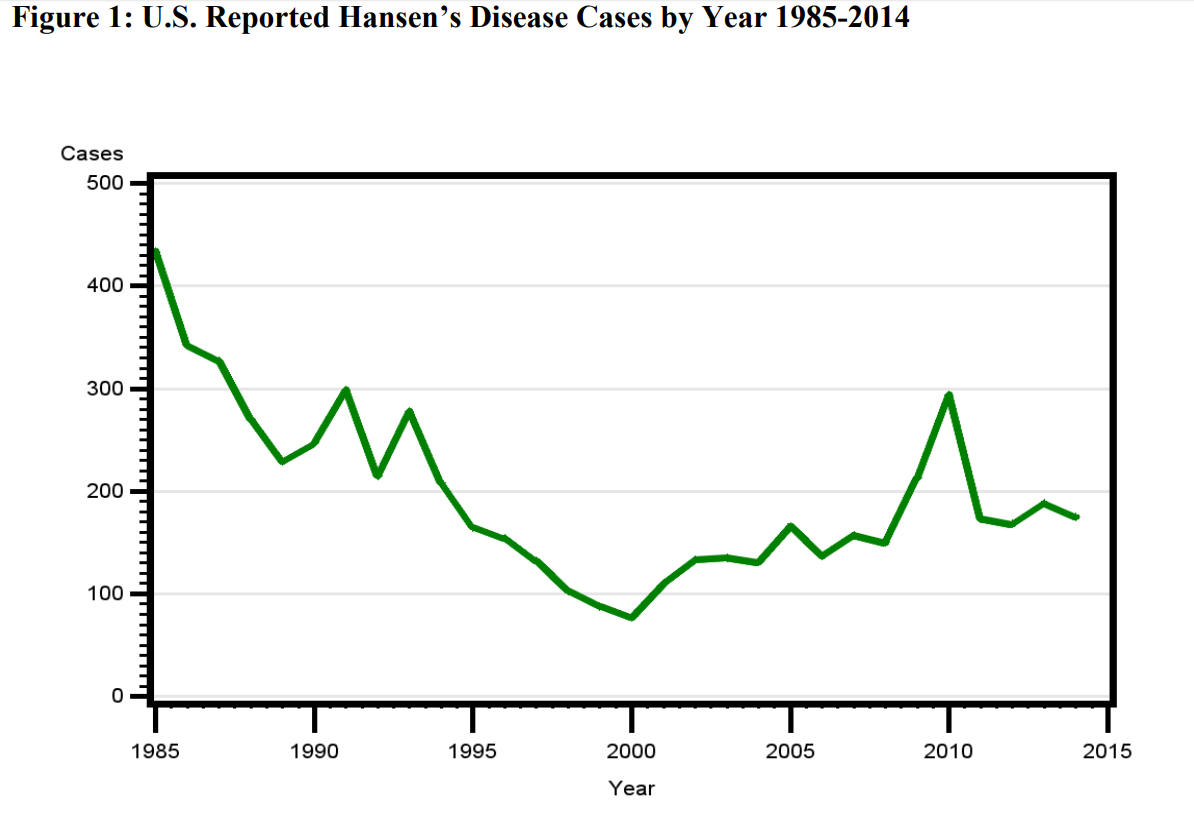
\includegraphics[width=1.0\textwidth,keepaspectratio]{hansen-incidence-USA.png}
	\end{frame}

	\begin{frame}
		\frametitle{Demographics in MA}
		\centering
		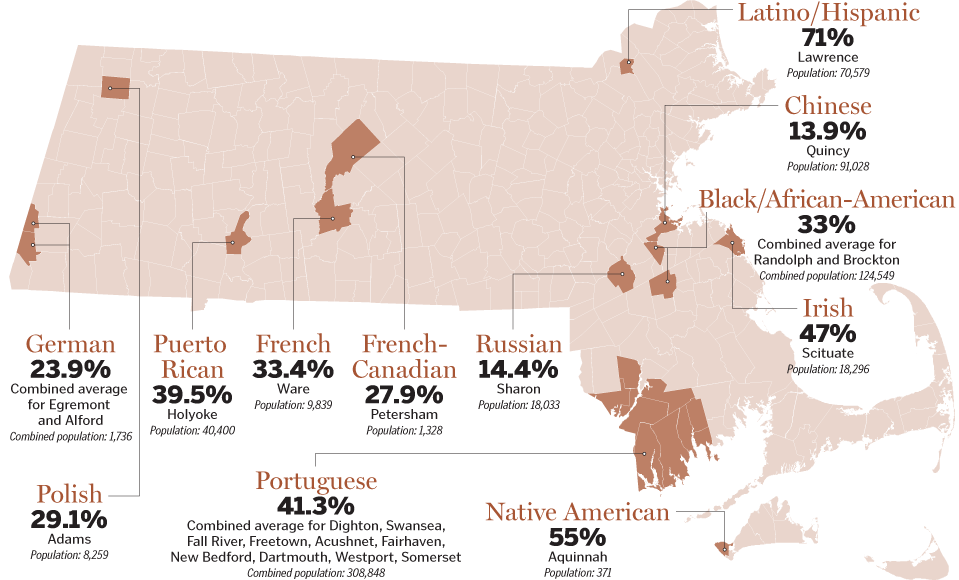
\includegraphics[width=1.0\textheight]{ma-immigration.png}
		
	\end{frame}

	\begin{frame}
		\frametitle{Incidence\textemdash Worldwide}
		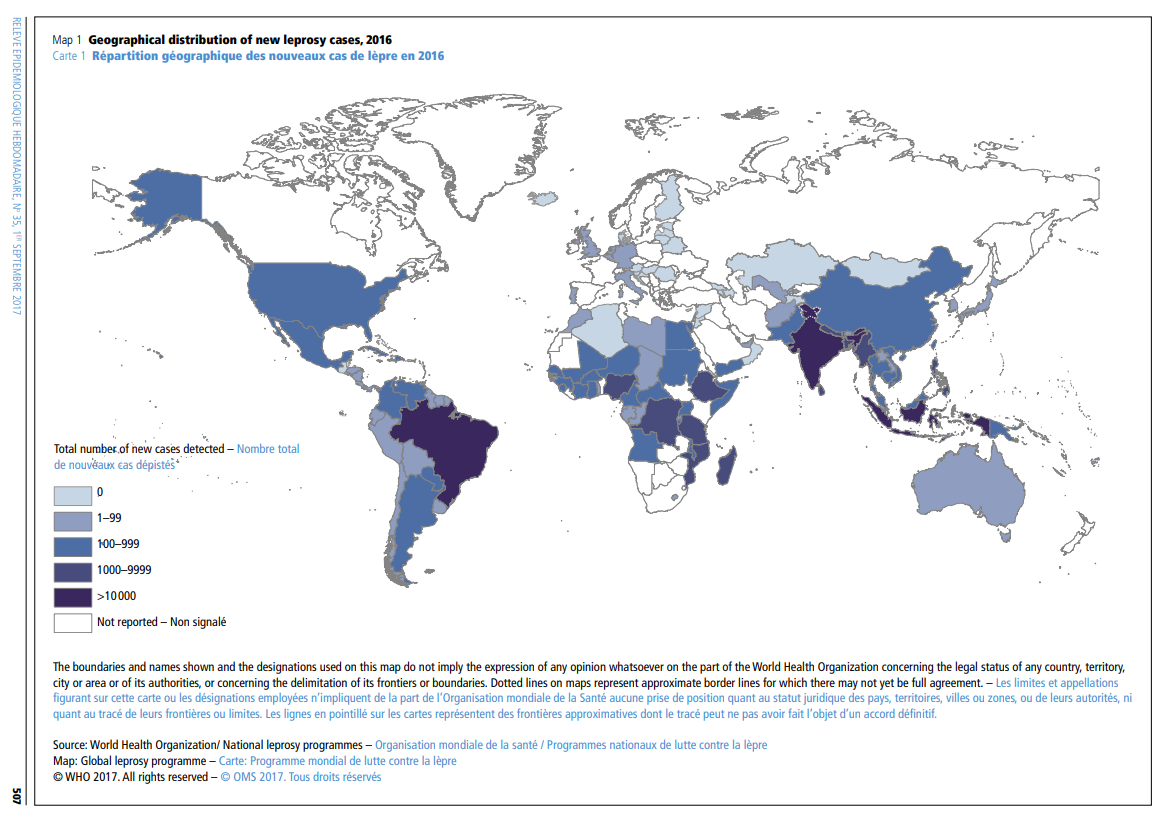
\includegraphics[width=1.0\textwidth,keepaspectratio]{hansen-incidence-world.png}
	\end{frame}
\section{Clinical Manifestations}
\subsection{Sites of Manifestation}
	\begin{frame}
		\frametitle{Sites of Manifestation}
			\centering
			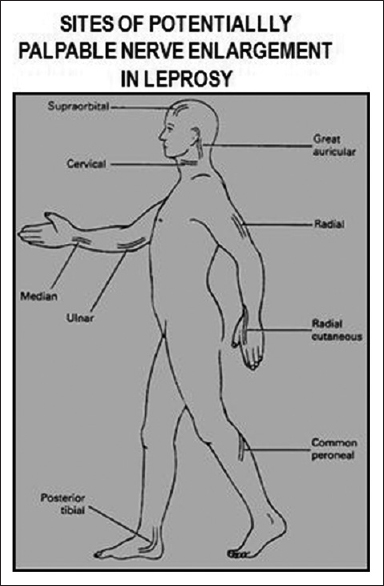
\includegraphics[height=0.90\textheight,keepaspectratio]{hansen-sites.jpg}
	\end{frame}

\subsection{Examples of Palpable Nerves}
	\begin{frame}
		\frametitle{Palpable (and Visible) Neuritis}
		\centering
		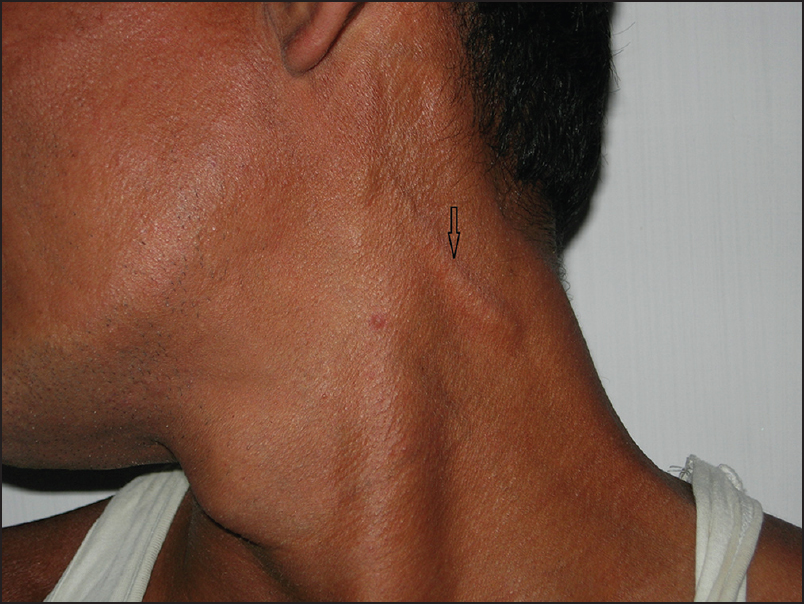
\includegraphics[height=0.8\textheight,keepaspectratio]{great-auricular.jpg}
	\end{frame}

	\begin{frame}
		\frametitle{Palpable (and Visible) Neuritis}
		\centering
		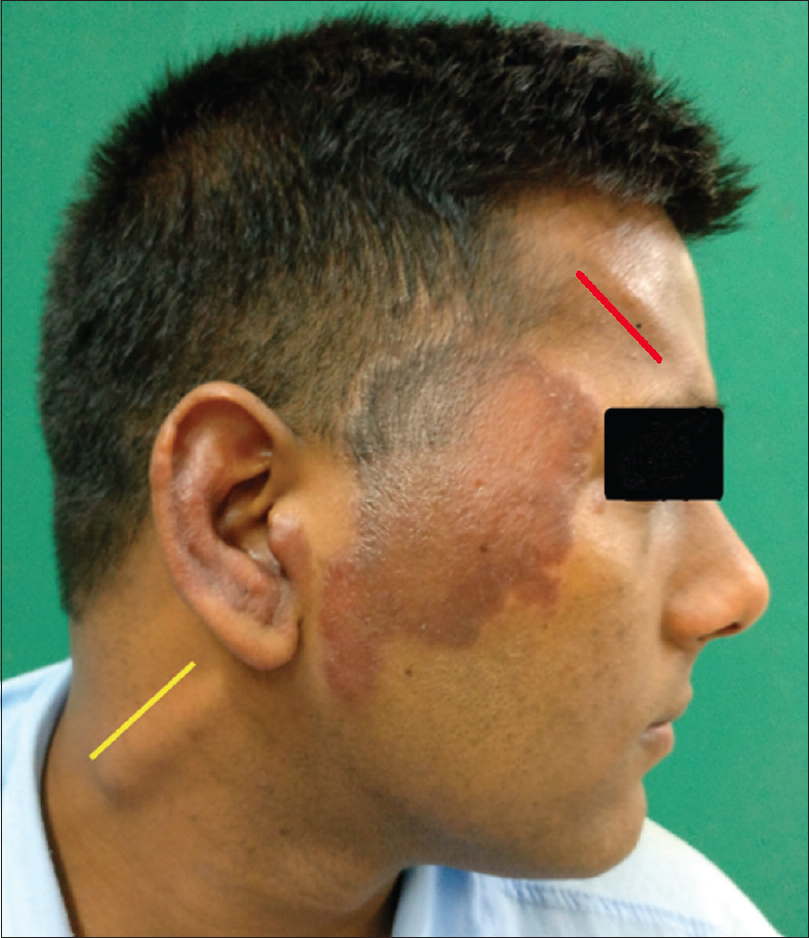
\includegraphics[height=0.8\textheight,keepaspectratio]{great-auricular-supraorbital.jpg}
	\end{frame}
	\begin{frame}
		\frametitle{Multiple Nerves}
		\centering
		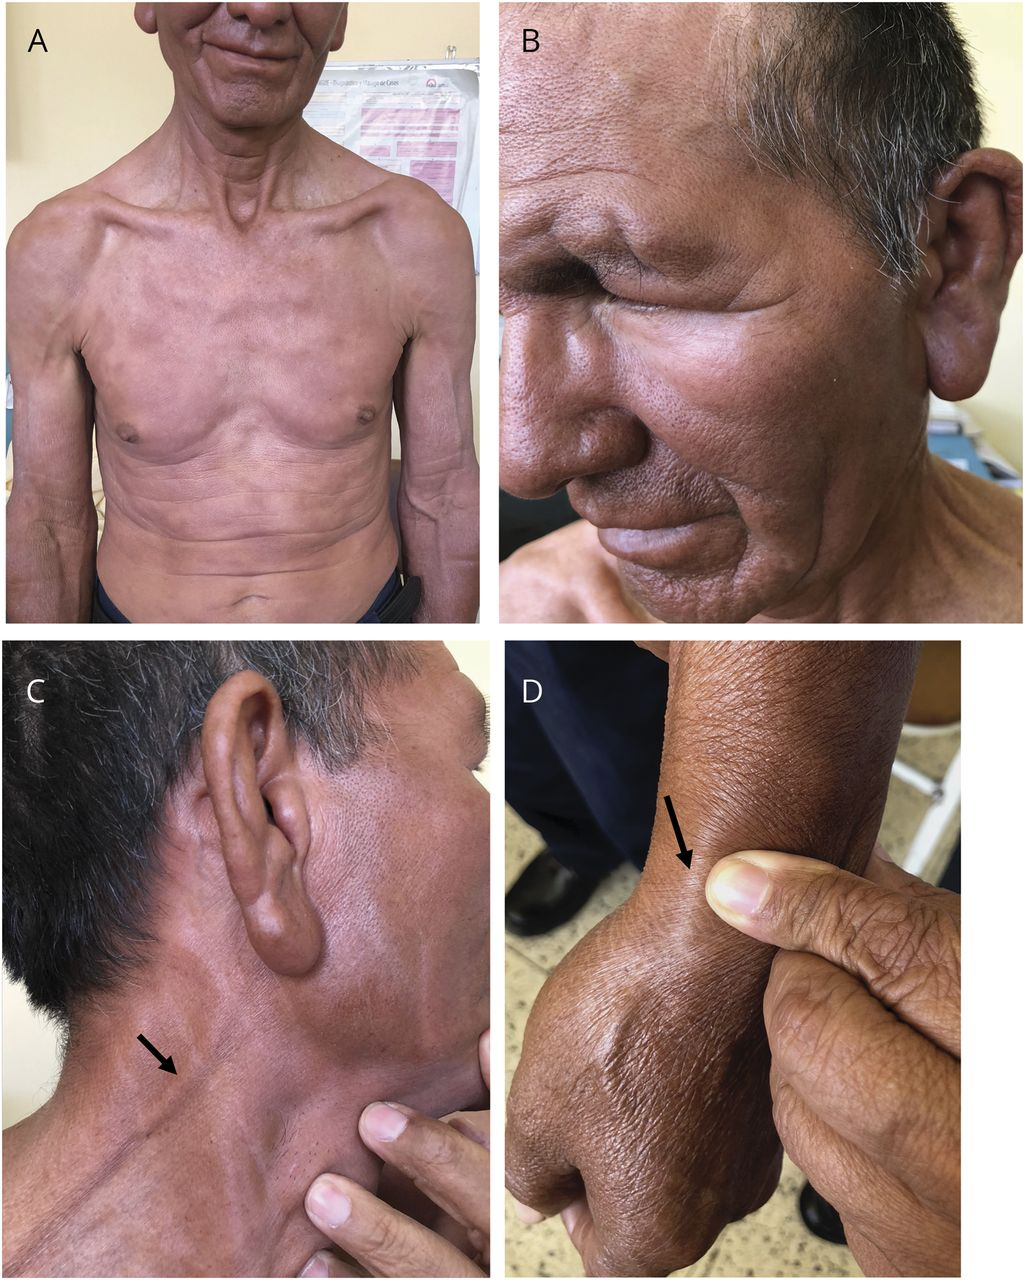
\includegraphics[height=0.8\textheight,keepaspectratio]{hansen's-overall.jpg}
	\end{frame}
       
	\begin{frame}
		\frametitle{Facial Nerve Palsy}
		\centering
		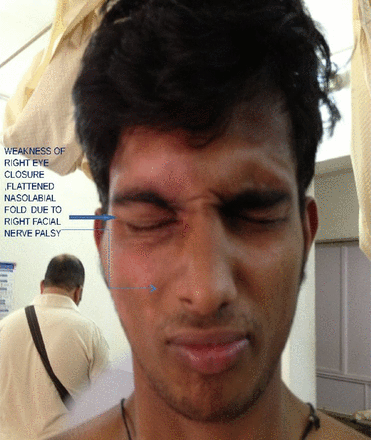
\includegraphics[height=0.8\textheight,keepaspectratio]{facial-palsy.png}
	\end{frame}

	\begin{frame}
		\frametitle{Anesthetic Hypopigmented Plaques}
		\centering
		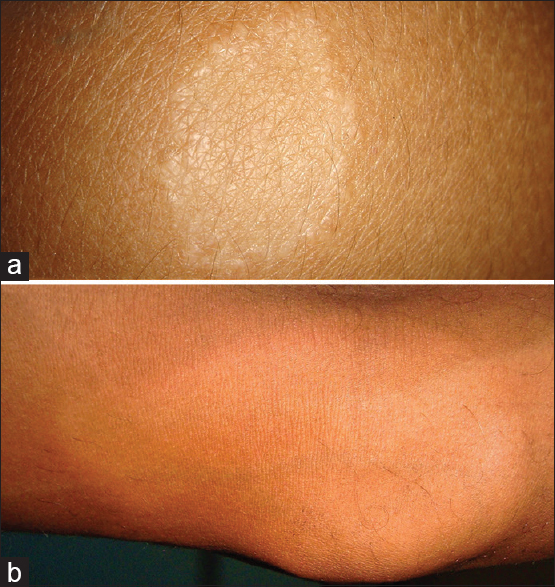
\includegraphics[height=0.8\textheight,keepaspectratio]{hypopigmented-plaques.jpg}
	\end{frame}

\subsection{Dermatologic Findings}
	\begin{frame}
		\frametitle{Erythema Nodosum Leprosum}
		\centering
		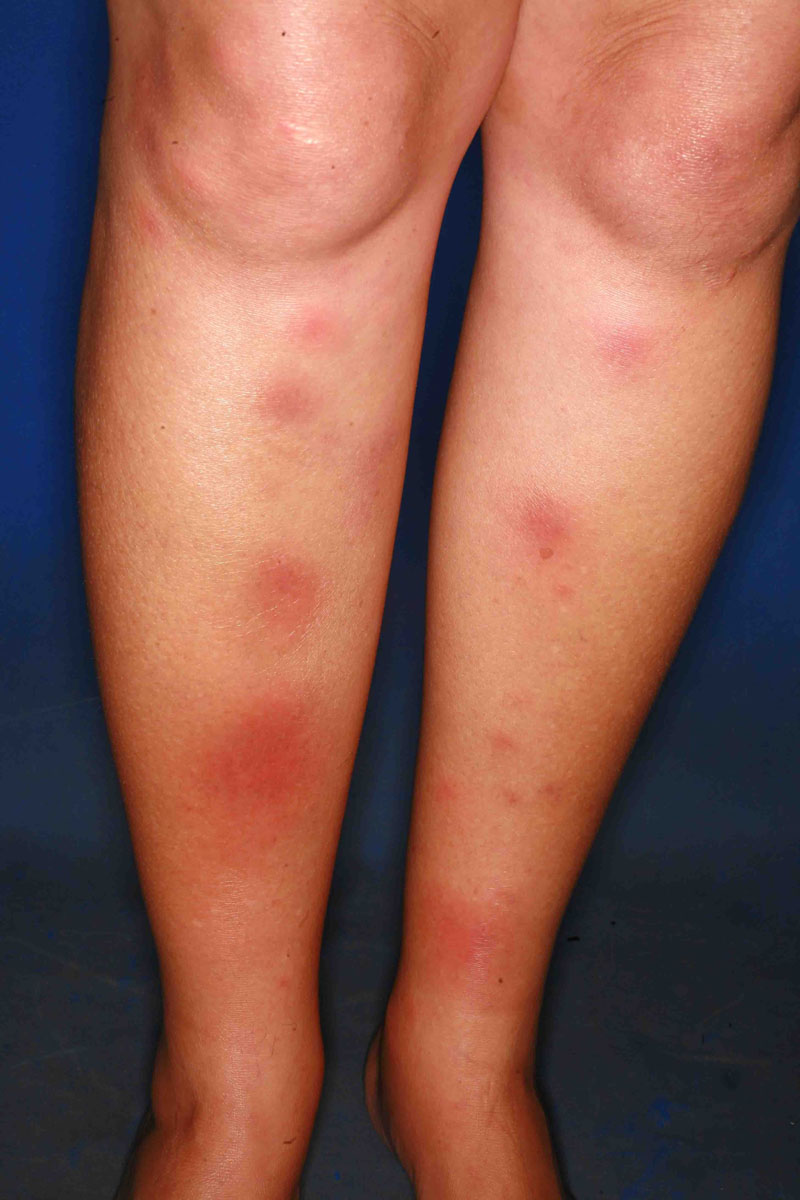
\includegraphics[height=0.8\textheight,keepaspectratio]{ENL.jpg}
	\end{frame}
\section{Diagnosis}
%\subsection{Ultrasound}
\subsection{Biopsy}
	\begin{frame}
		\frametitle{Findings on Biopsy}
		\centering
			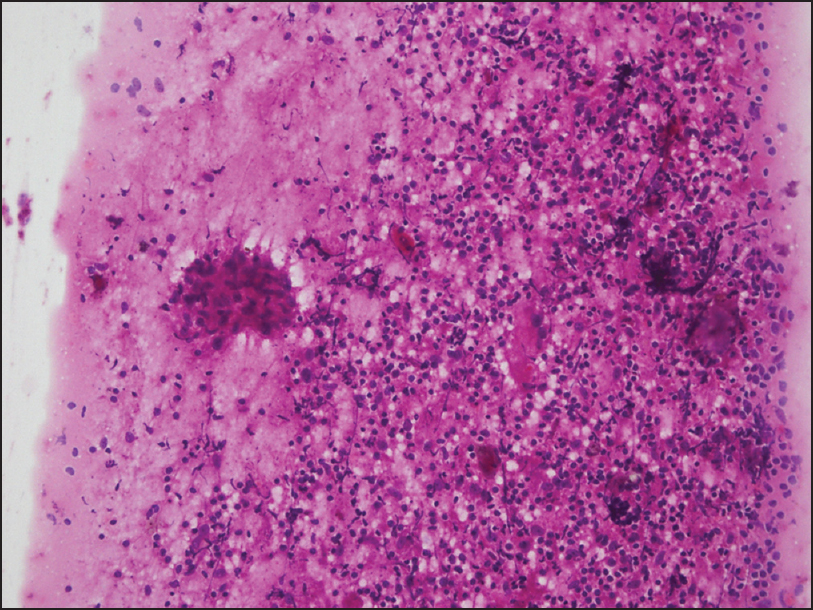
\includegraphics[height=0.40\textheight,keepaspectratio]{nerve-biopsy-hansens.jpg}
			\begin{columns}
				\column{0.5\textwidth}
				\centering
				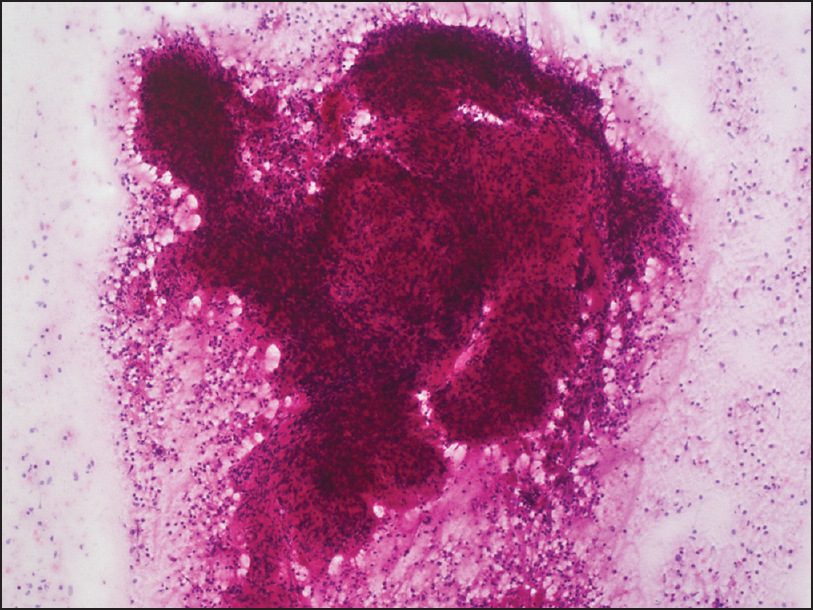
\includegraphics[height=.4\textheight,keepaspectratio]{nerve-aspirate-hansens.jpg}
				\column{0.5\textwidth}
				\centering
				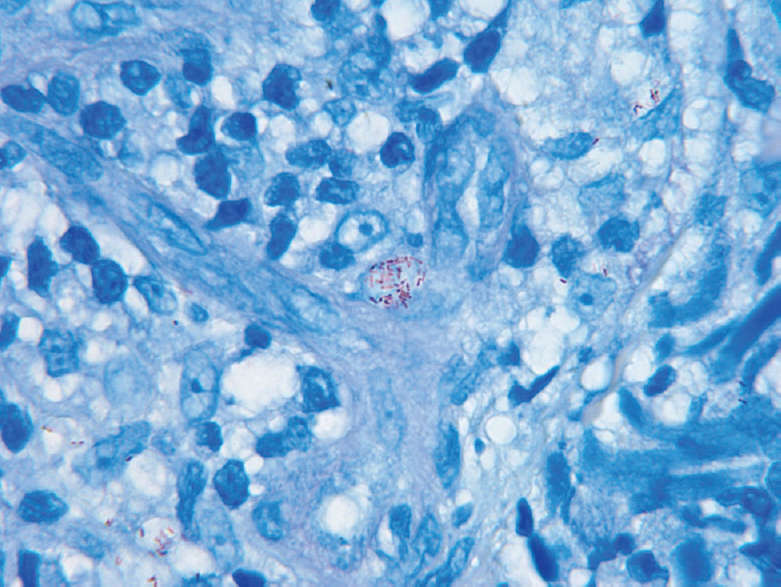
\includegraphics[height=.4\textheight,keepaspectratio]{fite-stain.jpg}
			\end{columns}
	\end{frame}
\section{Treatments}
\subsection{Antimicrobials}
	\begin{frame}
	\frametitle{Treatment\textemdash Antimicrobials}
		\begin{center}		
		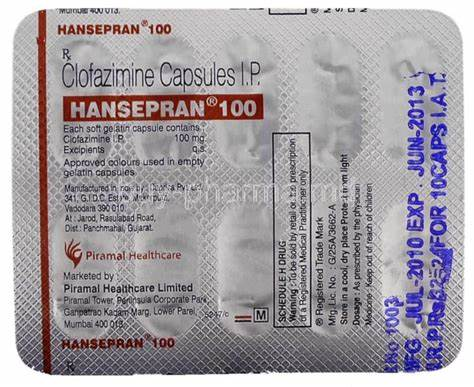
\includegraphics[height=0.35\textheight,keepaspectratio]{clofazimine-02.jpeg}
		\begin{columns}
			\column{0.5\textwidth}
			\centering
			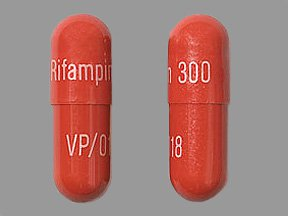
\includegraphics[height=.33\textheight,keepaspectratio]{rifampin.jpg}
			\column{0.5\textwidth}
			\centering
			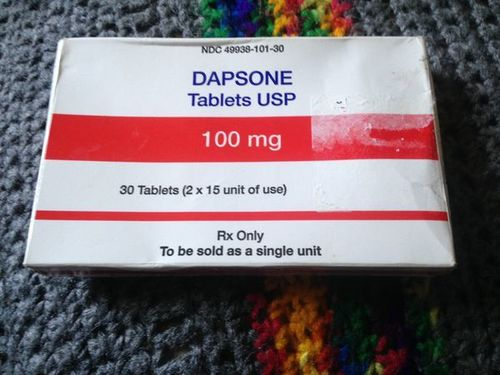
\includegraphics[height=.33\textheight,keepaspectratio]{dapsone.jpg}
		\end{columns}
	\end{center}
	\tiny
		{
			Images from: \href{https://www.webmd.com/drugs/2/drug-1744/rifampin-oral/details}{WebMD.com}, \href{https://www.buy-pharma.md/img/uploads/4264-hansepran-generic-lamprene-clofazimine-100-mg-packaging.jpg}{Buy-Pharma.md}
		}
	\end{frame}
\subsection{Immunosuppression}
	\begin{frame}
		\frametitle{Treatment\textemdash Neuritis}
			\begin{itemize}
				\item Type 1 Reactions (a.k.a. reversal reactions)
					\begin{itemize}
						\item First line: prednisone 40\textendash60 mg/day
						\item Second line: cyclosporine
						\item Unable to take steroids: MTX
					\end{itemize}
				\item Type 2 Reactions (a.k.a. ENL)
					\begin{itemize}
						\item Erythema nodosum leprosum
					\end{itemize}
			\end{itemize}
		\pause
		\begin{center}
			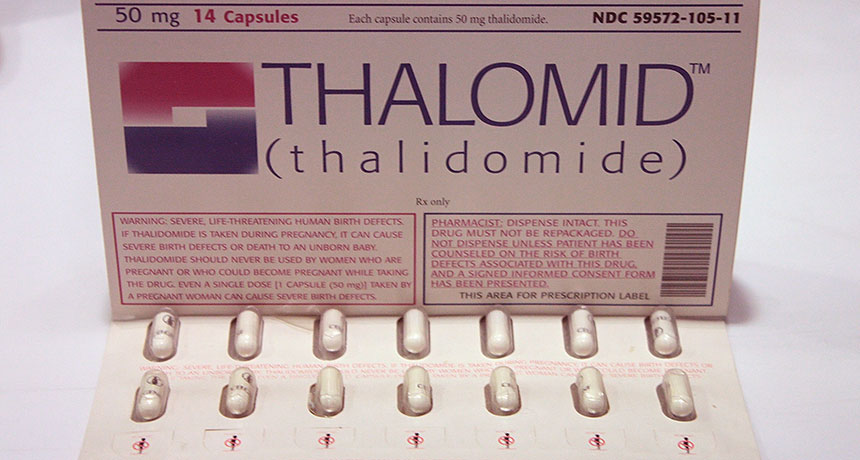
\includegraphics[width=0.6\textwidth,keepaspectratio]{thalidomide.jpg}
		\end{center}
		\tiny
			{
				Image from:
					\href{https://commons.wikimedia.org/wiki/File:Pack\_of\_Thalidomide\_tablets.jpg}{Wikimedia Commons}
			}
		\end{frame}
\end{document}
